\label{sec:vw}

In Section~\ref{cha:introduction}, we introduced the concept of \emph{virtual workspaces}. In this section we provide a more in--depth description of the term virtual workspace, a discussion of why virtual machines are a promising vehicle for virtual workspaces, and approaches to implementing workspaces, including the Globus Toolkit 4 \cite{DBLP:conf/npc/Foster05,globusweb} Workspace Service, on which we build upon in our work.

Virtual workspaces were first introduced by Keahey et al.\cite{VirtualWorkspaces05} as an abstraction for execution environments that can be deployed on a grid. This construct does not arise as a replacement for other execution management approaches, such as the widespread \emph{job} abstraction. Rather, it is a more general abstraction adequate for use cases requiring \emph{dynamic} and \emph{secure} deployment of execution environments (see Section~\ref{cha:scenarios}). This deployment can be dynamic if the user needs the execution environment to be created and destroyed on--demand, and it must be secure because both the software environment contained in the workspace and the user creating/managing/accessing the workspace must be trustworthy.

The two distinguishing aspects of virtual workspaces are:

\begin{description}
\item[Environment definition] or \emph{Quality of Life}: Workspaces provide an execution environment meeting all the software requirements of a user.
\item[Resource allocation] or \emph{Quality of Service}: All the resources the workspace needs to function correctly (CPU, memory, disk, bandwidth) must be provisioned and guaranteed during an agreed--upon availability period, allowing for dynamic renegotiation to reflect changing requirements and conditions.
\end{description}

The idea of on--demand creation and management of execution environments is not a new one, and there are multiple approaches to this problem, such as cluster node imaging (e.g. Cluster--on--Demand \cite{codweb}), configuration management (e.g. bcfg2 \cite{bcfg2web}), or package management (e.g. Pacman \cite{pacmanweb}). However, these approaches are not adequate for the stated goals. From the quality of life perspective, cluster node imaging and configuration management limit the software environments the user can choose. From the quality of service perspective, deploying hard drive images to cluster nodes requires a preparation time during which those nodes will be unavailable, and package management takes a long time to install and configure all necessary packages to create a software environment. Switching between different software environments frequently is, therefore, not cost--effective since resources cannot be used for computation while a new environment is being set up. Furthermore, none of these approaches support enforceable fine--grained resource allocation.


\section{VM--based Virtual Workspaces}
\label{sec:vm}

The use of virtualization technologies \cite{vmbook} holds great potential for Grid Computing. Figueiredo et al.\cite{gridvm} outlined several general advantages of using virtual machines in the context of Grid Computing. We are interested, in particular, in the following:

\begin{description}
\item[Security and isolation:] Virtualization isolates the actions performed in one VM from other VMs running in the same physical machine. Thus, VMs add an extra layer that must be broken by malicious grid users before the performance of co--allocated VMs can be affected, and before physical resource integrity can be compromised. Furthermore, users can be granted administrator privileges inside a virtual machine, since any malicious activity will be confined to the virtual machine, and will not affect the underlying physical machine \footnote{Granting administrator privileges can still enable malicious users to initiate attacks that require ``root'' access (such as a denial--of--service attack by flooding the network with packages, something which a non-privileged user user cannot do). Granting administrator privileges inside a virtual machine is, nonetheless, preferable to granting them on a physical machine, as system administrators can easily shut down malicious virtual machines without affecting any co--allocated virtual machines.}.
\item[Customization of execution environment:] Virtual machines can be customized with specific software and hardware requirements, without restarting physical nodes. Switching from one execution environment only requires starting a new virtual machine with the desired software environment, already preconfigured inside the virtual machine, instead of setting up a new environment from scratch, potentially removing the previous environment. This makes frequent switching between multiple execution environments a cost--effective option, requiring minutes instead of hours.
\item[Resource control:] Virtual machines enable enforceable fine--grained resource allocations that can be specified when creating the virtual machine, but also modified during the virtual machine's runtime. The resource enforcement mechanisms of virtual machines allow administrators to limit the impact of a VM's resource consumption on other co--allocated virtual machines, and also enables fine--grained accounting of resource usage. 
\item[Site-independence:] Virtual machines are very loosely coupled to physical hosts, only requiring that a host have an adequate virtual machine monitor and sufficient resources to support its execution. This enables virtual machines to be instantiated in different sites, imposing fewer constraints on the physical configuration of the site. Furthermore, virtual machines can be seamlessly migrated from one site to another.
\end{description}

Quality of life and service in virtual workspaces can be enhanced by leveraging these advantages. Security, isolation, and resource control positively affect quality of service by guaranteeing that workspaces have enough resources (CPU, memory, etc.) to support their execution, while being isolated from the resource usage of other co--located workspaces. Site--independence can improve quality of service by increasing the pool of physical resources where a workspace can run, and enabling cross--domain load balancing of workspaces. Customization, legacy support, and administrator privileges provide the users with quality of life, by decoupling them from the software environment provided by a resource provider and enabling them to specify custom software environments inside a virtual machine.

Virtual machine (VM) technologies  are, thus, a promising vehicle for achieving high quality of life and service in virtual workspaces. In a VM--based virtual workspace, the software environment required by the user would be encapsulated inside a virtual machine, and resource allocations would be enforced by a virtual machine manager.

\section{Representation of VM--based Virtual Workspaces}
\label{sec:vwrepresentation}

\begin{figure}
  \begin{center}
    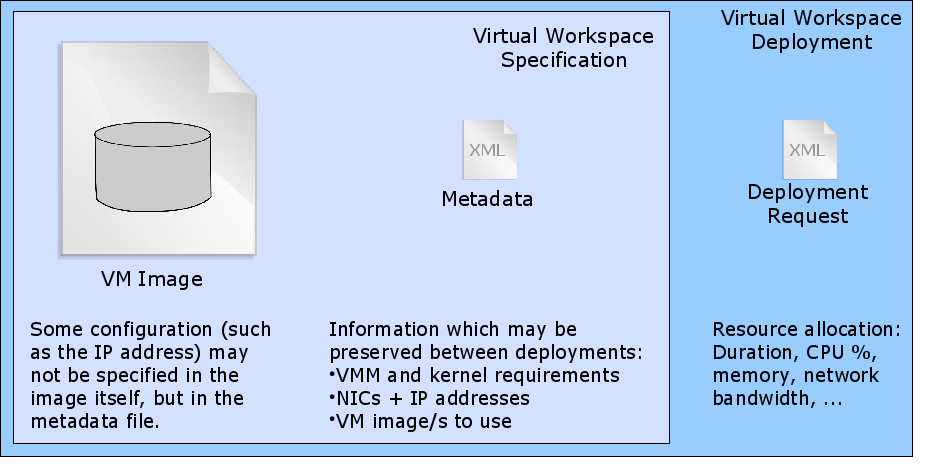
\includegraphics[width=0.85\textwidth]{figures/vw_representation.png}
    \caption{Virtual Workspace Representation}
	\label{fig:vwrepresentation}
  \end{center}
\end{figure}


A VM--based virtual workspace is composed of two elements \cite{VirtualWorkspaces05}, summarized in Figure~\ref{fig:vwrepresentation}, the \emph{VM image} and the \emph{workspace metadata}.

In a VM-based virtual workspace deployment, one or more virtual machines will be run. To instantiate a virtual machine, we need a \emph{disk image} with a runnable operating system and all the software required by the user. A VM image is composed of one or more disk images, representing the different disk partitions required by the virtual machines. Users could potentially provide their own VM images, or choose from a set of preexisting images made available by a resource provider.

Deployment--independent configuration information is factored out of the VM image and into an XML \emph{metadata file}. This approach allows workspaces to be described in terms of \emph{VM image templates}, generic reusable VM images with the system software and tools for some specific purpose (e.g. a worker node for an Open Science Grid cluster), but lacking all the configuration information specific to a particular type of deployment. This information, contained in the metadata file, is \emph{bound} to the VM image at runtime to produce an \emph{image instance}.

To illustrate the concept of image templates and why information in the metadata file is deployment--independent we present the following example:

\begin{enumerate}
\item A user wishes to deploy a virtual workspace representing an Open Science Grid (OSG) cluster with 100 worker nodes (for the purposes of this example, we will ignore the head node and focus only on the worker nodes). We assume that worker nodes differ only in their network configuration, and that the user wants to specify a single private IP address for each worker node manually (and not rely on other mechanisms, such as DHCP). Since each worker node will have a different network configuration, the user could prepare 100 worker node images, $W_1\ldots W_{100}$, that differ only in their network configuration. By using image templates and metadata files, the user only needs to provide a \emph{single} VM image $W$ and a metadata file $mf$ containing the network configuration of each of the worker nodes ($conf_1\ldots conf_{100}$).
\item When the virtual workspace is deployed, multiple copies of the image template are made, and each is bound to the configuration contained in the metadata file to produce runnable image instances (e.g. $W(conf_{42})=W_{42}$). Note that the image template is reusable, since a single copy of an image template can be used to yield multiple image instances.
\item Metadata file $mf$ can be reused for future deployments of a 100--node OSG cluster. In this sense, the configuration information contained in the metadata file is \emph{deployment--independent}.
\item In the future, the user wishes to deploy a 150--node cluster, using the same VM image $W$. Metadata file $mf$ cannot be used as it only includes configuration for 100 nodes. To deploy the new workspace, the user must create a new metadata file, $mf'$, with configuration information for all the nodes ($conf_1\ldots conf_{150}$). Similarly, if the user wishes to deploy the 100--node cluster but using network addresses different from the ones specified in $mf$, a new metadata file would also be required. Therefore, we consider that any configuration information that \emph{need not} change across deployments is deployment--independent. Furthermore, this example also shows how an image template can be reused not just in a single deployment (by using it to create multiple image instances) but across deployments, since all potentially mutable information is contained in the metadata file, not in the VM image.
\end{enumerate}

In Section~\ref{cha:design} we will explore optimizations that result from the reusability of image templates.

Finally, when a virtual workspace is deployed, we must also specify a \emph{deployment request} (also shown in Figure~\ref{fig:vwrepresentation}). This request is an XML document describing the resource
allocation required by the workspace, including both availability and hardware requirements (such as memory and
CPU\%). This information is \emph{deployment--dependent}, since resource allocation requirements generally vary across deployments (e.g., the user might be interested in performing CPU--intensive work in one deployment, and I/O--intensive work in another), and also during a deployment (to adapt to changing requirements and conditions).


\section{GT4 Workspace Service}

\begin{figure}
  \begin{center}
    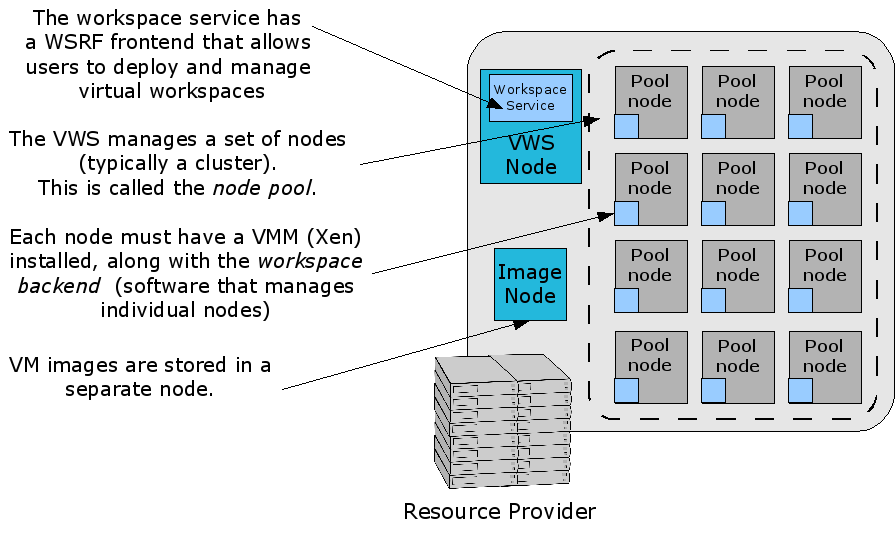
\includegraphics[width=\textwidth]{figures/vw_overview.png}
    \caption{Virtual Workspace Service}
	\label{fig:vwservice}
  \end{center}
\end{figure}


The GT4 Virtual Workspace Service \cite{vwsweb}, or VWS, which we extend in this work, allows authorized users to request the creation of VM--based virtual workspaces through a Web Services interface. This interface also allows users to monitor and control the virtual workspace. As of this writing, the VWS only supports single--node virtual workspaces and immediate reservations without the possibility of queueing or preemption (i.e. requests for which resources cannot be provisioned immediately  are rejected). Virtual machines are instantiated using the Xen Virtual Machine Monitor \cite{xen}, although others (such as VMWare \cite{vmwareweb}) could potentially be used.

Figure~\ref{fig:vwservice} shows the typical setup required by the VWS in the resource provider:

\begin{itemize}
\item A publicly accessible node, the \emph{VWS node}, hosts the Web Service frontend of the VWS.
\item A set of nodes, the \emph{node pool} are put under the control of the VWS. Virtual workspaces will be deployed on these nodes.
\item Each node in the node pool must have a virtual machine manager installed, along with the \emph{workspace backend}, a script that manages individual nodes and is invoked by the VWS when tasks need to be performed on nodes (such as starting and stopping virtual machines.
\item A separate node, the \emph{image node} acts as a repository for VM images. When a virtual workspace is deployed on the node pool, VM images are staged to the nodes from the image node.
\end{itemize}

In a typical interaction with the VWS, the following steps would take place:

\begin{enumerate}
\item A user wishes to deploy a virtual workspace. To do so, the user provides the location of the VM image (in either the image node or a third--party site), the workspace metadata, and the deployment request (as described in the previous section).
\item The VWS determines if there are enough resources immediately available to satisfy the request. If not, the request is rejected. Otherwise, the VWS initiates a transfer of the VM image to the nodes where that VM image will be used.
\item Once the image transfer is completed, the VWS uses the workspace backend to start the virtual machines for the requested workspace.
\item Information about the workspace, such as its status, the IP addresses assigned to the virtual machines, etc. are published through the Web Services interface, using WSRF Resource Properties.
\item Users can query these Resource Properties, and interact with their workspaces in the same way they would with a physical machine.
\item Users can also use the Web Services interface to control their workspaces (e.g. to stop them when they are done with their work)
\end{enumerate}
